\documentclass{article}

% Langue française et codage
% \usepackage[T1]{fontenc}
% \usepackage[utf8]{inputenc}
% \usepackage[french]{babel}

% pour les symboles et opérations mathématiques
\usepackage{amsmath, amssymb, amsthm} 

% Styling
\usepackage[letterpaper, top = 2cm, bottom = 2cm, right = 2cm, left = 2cm, heightrounded]{geometry}

\usepackage{fancyhdr} %header and footer

\pagestyle{fancy}
\fancyhf{}
\fancyhead[L]{\leftmark}
\fancyhead[C]{Hafid} % Ou un nom en texte brut
\fancyfoot[R]{\thepage}

\usepackage{subfiles}

% Figures
\usepackage{graphicx, float} % images
\graphicspath{img/} % path

\usepackage{tikz, pgfplots}
\pgfplotsset{compat=1.18, trig format plots=rad}
\usetikzlibrary{arrows.meta, positioning, calc, shapes, decorations.pathmorphing, patterns, 3d}


\usepackage{hyperref, cleveref} % references
\hypersetup{
    colorlinks=true,
    linkcolor=black,     % Color for internal references (\ref, \cite)
    citecolor=black,     % Color for citations
    urlcolor=blue        % Color for external websites (\url, \href)
}

\usepackage{booktabs} % tableaux

\usepackage{lipsum} % lorem ipsum

\usepackage[style=numeric, backend=biber]{biblatex}
\addbibresource{biblio.bib}


\linespread{1.15} % espacement des lignes
% \setlength{\parskip}{0.8em}

\hbadness=10000 % avoid error

\title{Linear Transformations}
\author{Hafid}
\date{\today}


% theorems
\newtheorem{theorem}{Theorem}[section] % numorezation : [chapter]


\theoremstyle{definition}
\newtheorem{definition}[theorem]{Definition}

\theoremstyle{remark}
\newtheorem{remark}[theorem]{Remark}

\newtheorem{prop}[theorem]{Properties}

\newtheorem{lemma}{Lemma}
\newtheorem{corollary}{Corollary}

\counterwithin*{section}{part}
% \counterwithin*{theorem}{section}
\numberwithin{equation}{section}

\newcommand{\N}{\mathbb{N}}
\newcommand{\Z}{\mathbb{Z}}
\newcommand{\Q}{\mathbb{Q}}
\newcommand{\R}{\mathbb{R}}
\newcommand{\C}{\mathbb{C}}
\newcommand{\K}{\mathbb{K}}
\newcommand{\mat}[2]{\mathcal{M}_{#1} (#2)}
\NewDocumentCommand{\lt}{o o}{
    \IfNoValueTF{#1}{\mathcal{L} (E, F)}
        {\IfNoValueTF{#2}{\mathcal{L} (#1)}
            {\mathcal{L} (#1, #2)}
    }
}

\begin{document}
\maketitle
\tableofcontents

\section{Definition}

    \begin{definition}
        \(f : E \to E, x \to f(x)\) \\
        \(f\) a is Linear Transformation \(\iff \forall x, y \in E, \forall \lambda \in \mathbb{R} : f(\lambda x + y) = \lambda f(x) + f(y)\) \\
        We denote the set of linear applications as: \( \lt \) and \( \lt{E}\) if \(f : E \to E\)
        \begin{align}
        \text{f is a homomorphism} &\iff \text{f is LT}\label{eq:homo}\\
        \text{f is a endomorphism} &\iff \text{\eqref{eq:homo}  and } f  : E \to E\label{eq:endo} \\
        \text{f is an isomorohism} &\iff \text{\eqref{eq:homo}  and $f$ is bijective}\label{eq:ismo}\\
        \text{f is an automorphism} &\iff \text{\eqref{eq:homo} and~\eqref{eq:endo} and~\eqref{eq:ismo}}
        \end{align}
    \end{definition}

    \begin{prop}
        \(f\) is a linear transformation, then:
        \begin{itemize}
            \item \(f(0_{E}) = 0_{F}\)
            \item \(f(-x) = - f(x)\)
        \end{itemize}
    \end{prop}

\section{Kernel, Image and morphisms}
\begin{remark}
    \(f\) is a linear transformation in the following:
\end{remark}

\begin{definition} (Kernel)
    \( \ker f = \{x \in E \mid  f(x) = 0_{E}\} \)
\end{definition}

\begin{theorem}
    f is injective \(\iff \ker f = \{0_{e}\} \iff \dim{(\ker f)} = 0\)
\end{theorem}

\begin{definition} (Image)
    \(\mathrm{Im}f = \{f(x) \mid  x \in E\}\)
\end{definition}

\begin{theorem}
    f is surjective\(\iff \mathrm{Im}f = F \iff \dim{(\mathrm{Im} f)} = \dim{F}\) 
\end{theorem}

\begin{theorem}
    f is bijective \(\iff\) f is injective and surjective.
\end{theorem}

\begin{prop}
    \( \dim{E} = \dim{\ker f} + \dim{\mathrm{Im}f}\)

\end{prop}

\begin{theorem}
    If E = F then:\\
    f is injective 
    \(\iff\) f is surjective 
    \(\iff\) f is bijective
    \(\iff \ker{f} = \{0_{E}\}
    \iff \mathrm{Im}f = E
    \iff \dim{\ker{f}} = 0
    \iff \dim{\mathrm{Im}f} = \dim{E}\)
\end{theorem}






\section{Matrices associated with linear transformation}

\begin{definition}
    Let $B = \{e_{1}, e_{2}, \dots, e_{n}\}$ a basis of $E$ 
    and $B'= \{e_{1}', e_{2}', \dots, e_{p}'\}$ a basis of $F$,
    Then the associated matrice of the LT $f$ is given by:
    \[ Mat = 
        \bordermatrix{
            ~      & f(e_{1})   & f(e_{2})    & \cdots  & f(e_{n}) \cr
            e_1    & \alpha_{1} & \alpha_{1}' & \cdots  & \alpha_{1}^{(p)} \cr
            e_2    & \alpha_{2} & \alpha_{2}' & \cdots  & \alpha_{2}^{(p)} \cr
            \vdots & \vdots     & \vdots      & \ddots & \vdots \cr
            e_n    & \alpha_{n} & \alpha_{n}' & \cdots  & \alpha_{n}^{(p)}
        }
    \]
    \begin{remark}
        Writing $f(e_{k})$ as 
        $f(e_k) = \alpha_{1}^{(k)}e_{1}'+\alpha_{2}^{(k)} e_{2}' 
        + \cdots + \alpha_{n}^{(k)} e_{n}'$ 
        then write the coefs in columns\\
        (\(\alpha_n^{(k)}\) means  \(\alpha\) k-times prime)
    \end{remark}

    We denote ${Mat(f)}_{B_{1}, B_{2}}$ the matrix associated with the linear application $f : E \to F$ with the basis $B_{1}, B_{2}$ of $E, F$ respectively. 
    If $f : E \to E$ then we just denote it ${Mat(f)}_{B_{1}}$ or ${Mat(f)}$.
    \begin{remark}
        $f^n$ DOES NOT MEAN $f \times f \times \dots f$ n- times.\\
        It means $f\circ f\circ \dots \circ f$ (Composition of f with itself n-times)\\
        That composition becomes a matrice power Prop.~\ref{prop:5} 
    \end{remark}
     

\end{definition}

\begin{prop}
    \(\forall f, g \in \lt, \forall \lambda \in \mathbb{K}\)
    \begin{enumerate}
        \item \(Mat (\lambda f) = \lambda Mat (f)\)
        \item \(Mat (f + g) = Mat(f) + Mat(g)\)
        \item \(Mat (gof) = Mat(g) \times Mat(f)\)
        \item \(Mat (f^{-1}) = {Mat(f)}^{-1} \emph{\textbf{(very important)}}\)
        \item \(Mat (f^p) = {Mat(f)}^p\)\label{prop:5}
    \end{enumerate}
\end{prop}



\section{The change of basis:}

\begin{definition}
    Given a basis \(B_{1} = \{e_{1}, e_{2}, \ldots, e_{n}\}\) and a basis \(B_{2}=\{e_{1}', e_{2}', \dots, e_{n}'\}\) of the same set E.\\
    To find the transition matrice, you need to write each vector $e_k'$ as a linear compoision of the basis $B_1$\\
    \(e_{k}'=\alpha_{1}^{(k)}e_{1}+\alpha_{2}^{(k)}e_{2} + \cdots + \alpha_{n}^{(k)} e_{n}\)\\
    Then write the coefs in columns:
    \[P_{B_{1} \to B_{2}} = 
        \bordermatrix{
            ~ & e_1' & e_2' & \cdots & e_n' \cr
            e_1 & \alpha_{1}' & \alpha_{1}'' & \cdots & \alpha_{1}^{(k)} \cr
            e_2 & \alpha_{2}' & \alpha_{2}'' & \cdots & \alpha_{2}^{(k)} \cr
            \vdots & \vdots & \ddots & \vdots \cr
            e_n & \alpha_{n}' & \alpha_{n}'' & \cdots & \alpha_{n}^{(k)}
        }
    \]
    Let \(f : E \to F\) such that \(f \in \lt \) and \(B_{1}, B_{2}\) are basis of E and F resp.\\
    To find the linear transformation f in another base, we need to find the matrix associated with it in that matrix with the formula:
    \[{Mat(f)}_{B_{2}, B_{2}'} = P^{-1}_{B_{1} \to B_{2}} \times {Mat(f)}_{B_{1}, B_{1}'} \times P_{B_{1}' \to B_{2}'}\]
\end{definition}


\begin{figure}[H]
    \begin{center}
        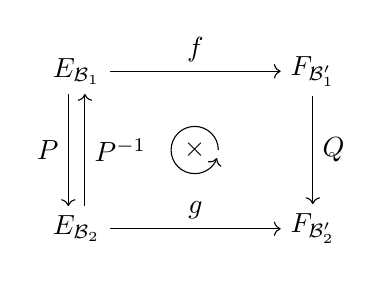
\begin{tikzpicture}
            \node (E1) at (0, 0) {$E_{\mathcal{B}_{1}}$};
            \node (F1) at (3, 0) {$F_{\mathcal{B}_{1}'}$};
            \node (E2) at (0, -2) {$E_{\mathcal{B}_{2}}$};
            \node (F2) at (3, -2) {$F_{\mathcal{B}_{2}'}$};
            \draw[->] (E1) -- node[above] {$f$} (F1);
            \draw[->] (E2) -- node[above] {$g$} (F2);
            \draw[->] ([xshift=-3pt]E1.south) -- node[left] {$P$} ([xshift=-3pt]E2.north);
            \draw[->] ([xshift=3pt]E2.north) -- node[right] {$P^{-1}$} ([xshift=3pt]E1.south);
            \draw[->] (F1) -- node[right] {$Q$} (F2);

            \draw[->] (1.8, -1) arc(0:340:0.3);
            \node (x) at (1.5, -1) {$\times$};

        \end{tikzpicture}
    \end{center}
    \caption{Change of basis Diagram}
\end{figure}

Such that $P$ is the transformation matrix from $B_{1} \to B_{2}$ and $Q$ from $B_{1}' \to B_{2}'$.\\
and we write ${Mat(f)}_{B_{1}', B_{2}'} = P^{-1}\times {Mat(f)}_{B_{1}, B_2}\times Q$


\begin{prop}
    $f : E \to E \implies {Mat(f)}_{B_{1}'} = P^{-1}\times {Mat(f)}_{B_{1}}\times P$
\end{prop}

\begin{prop}
    ${Mat(f)}_{B_{1}', B_{2}'}^n = P^{-1}\times {Mat(f)}^n_{B_{1}, B_{2}}\times P$
\end{prop}
\end{document}